% =====================================================================
% 06_muestreo.tex
% Metodología estadística del muestreo: EDA, post-estratificación y GREG
%
% Fuente: 03_informes/analisis_fase2/metodologia_muestreo.md (2026-10-14),
% generado por documentacion_auditoria/src/generar_metodologia_muestreo.py a
% partir de data/memoria/eda_resultados.json, data/memoria/estimadores_resultados.json
% y data/memoria/diagnosticos_greg.json.
%
% Las cifras son las mismas del informe: no se recalculó nada al pasar a LaTeX.
% =====================================================================

\section{Muestreo y estimación del análisis longitudinal}
\label{sec:muestreo}

\textbf{Alcance.} Esta sección es un \emph{ejercicio metodológico}: documenta
\emph{cómo} se estimaría y qué se gana con cada estimador. Las cifras oficiales
del análisis longitudinal son las del \textbf{censo} (la base completa está
disponible) y se reportan en \texttt{analisis\_longitudinal.md}; aquí se usan
además como patrón de contraste, lo que permite verificar de verdad cada
estimador en lugar de confiar en la teoría.

\textbf{Datos.} 77 237 registros, 30 086 personas únicas y 6 convocatorias
(2013--2021). Muestra vigente: 2 224 personas, muestreo aleatorio simple (MAS)
con semilla 2026.

% =====================================================================
\subsection{Marco teórico}
\label{sec:mues-marco}

\subsubsection{Por qué un EDA antes de decidir el muestreo}

El análisis exploratorio no es un trámite previo: es lo que permite elegir el
diseño. Como resume la literatura de muestreo, «el análisis exploratorio de
datos, incluidas la producción de resúmenes simples, tabulaciones y gráficos, es
normalmente la primera etapa de cualquier análisis de este tipo» y se debe
«llevar a cabo trabajo exploratorio sobre subconjuntos o muestras para
clarificar qué enfoque será a la vez práctico y eficaz» (StatsRef.com, sobre
Cochran, 1977). En este proyecto el EDA cumple tres funciones concretas:

\begin{enumerate}
  \item \textbf{Detectar si hay estratos naturales}, es decir, grupos con
        comportamiento muy distinto. Si no los hay, la estratificación no aporta
        y complica el diseño.
  \item \textbf{Detectar grupos pequeños} que necesitarían representación
        garantizada y no la tienen con un MAS.
  \item \textbf{Cuantificar la varianza intra e inter-grupo}, que es exactamente
        lo que determina cuánta precisión se gana al estratificar.
\end{enumerate}

\subsubsection{Los tres estimadores y su relación}

\begin{table}[H]
  \centering
  \small
  \caption{Los tres estimadores comparados.}
  \label{tab:mues-estimadores}
  \begin{tabular}{@{}p{3.1cm}p{5.3cm}p{6.6cm}@{}}
    \toprule
    \textbf{Estimador} & \textbf{Idea} & \textbf{Fundamento} \\
    \midrule
    \textbf{MAS (expansión simple)} & Cada persona entra con el mismo peso
      $N/n$ & Cochran (1977); Lohr (2010). Insesgado por diseño \\
    \textbf{Post-estratificado} & Se reponderan los pesos para que la muestra
      reproduzca la composición conocida de la población en categorías &
      Cochran (1977, §5A); Lohr (2010, §7.6). Su distribución asintótica
      coincide con la de un muestreo estratificado con asignación proporcional \\
    \textbf{GREG (model-assisted)} & Se usa un modelo de regresión como
      auxiliar, pero la validez de la estimación \textbf{no} depende de que el
      modelo sea correcto & Särndal, Swensson \& Wretman (1992, §6.4--6.5);
      FCSM (2003); Kalton (2002) \\
    \bottomrule
  \end{tabular}
\end{table}

La idea central del GREG es la del \textbf{modelo asistido}: el modelo se usa
para ganar eficiencia, no para sostener la inferencia. Como lo formulan Kalton
(2002) y el FCSM (2003), «los modelos se usan ampliamente dentro del modo de
inferencia basado en el diseño, tanto en el diseño muestral como en la
estimación, pero de manera asistida por el modelo, de forma que la validez de
las estimaciones no depende de la validez de los supuestos del modelo». La
propiedad que lo garantiza es la consistencia por diseño: si el modelo es malo,
el estimador sigue siendo aproximadamente insesgado porque el término de
corrección usa los residuos observados en la muestra.

Formalmente, con probabilidades de inclusión $\pi_i = n/N$ (MAS sin reemplazo)
el estimador de diferencia que se implementa aquí es

\begin{equation}
  \hat{Y}_{GREG} \;=\; \frac{1}{N}\sum_{i\in U}\hat{y}_i
  \;+\; \frac{1}{n}\sum_{i\in s}\left(y_i - \hat{y}_i\right)
  \label{eq:mues-greg}
\end{equation}

y con un modelo \textbf{lineal} adopta la forma clásica
$\bar{Y}_{GREG} = \bar{y}_s + (\bar{X}_U - \bar{x}_s)'\hat{\beta}_s$, donde las
medias de las auxiliares se conocen para \textbf{toda} la población. Un detalle
importante para interpretar los resultados: \textbf{la post-estratificación es
un caso particular de GREG} con un modelo saturado en los post-estratos. En la
sección~\ref{sec:mues-comparacion} se comprueba numéricamente.

% =====================================================================
\subsection{EDA: qué se exploró y qué se encontró}
\label{sec:mues-eda}

\subsubsection{Univariado}

\textbf{Categóricas} (perfil de cada persona en su última convocatoria
observada, $n = 30\,086$):

\begin{table}[H]
  \centering
  \small
  \caption{Distribución de las variables categóricas del censo.}
  \label{tab:mues-univariado}
  \begin{tabular}{@{}lrl@{}}
    \toprule
    \textbf{Variable} & \textbf{Categorías} & \textbf{Distribución} \\
    \midrule
    Categoría & 4 & Investigador Junior 68,7 \% · Investigador Asociado 19,2 \% ·
        Investigador Sénior 10,9 \% · Investigador Emérito 1,1 \% \\
    Género $\dagger$ & 3 & Masculino 60,6 \% · Femenino 39,4 \% ·
        Otro / No especificado 0,0 \% \\
    Gran área & 7 & Ciencias Sociales 30,7 \% · Ciencias Naturales 20,9 \% ·
        Ingeniería y Tecnología 18,7 \% · Ciencias Médicas y de la Salud 15,2 \% ·
        Humanidades 8,0 \% · \dots{} (7 en total) \\
    Nivel de formación & 10 & Doctorado 49,4 \% · Maestría/Magister 36,0 \% ·
        Postdoctorado 7,6 \% · Especialidad Médica 2,5 \% · Pregrado/Universitario
        2,2 \% · \dots{} (10 en total) \\
    Departamento & 35 & Bogotá D.~C. 32,6 \% · Antioquia 16,6 \% · Valle del
        Cauca 8,3 \% · Atlántico 6,2 \% · Santander 5,2 \% · \dots \\
    \bottomrule
  \end{tabular}

  \smallskip
  {\footnotesize $\dagger$ El género se presenta \textbf{colapsado}:
  \emph{Intersexual} (5 personas) y \emph{No disponible} (4) se agrupan en
  \emph{Otro / No especificado} (9 personas, 0,030 \% del censo) porque
  \textbf{ninguna de las dos aparece en la muestra}. La decisión y sus
  consecuencias se documentan en la
  sección~\ref{sec:mues-genero}.}
\end{table}

\textbf{Edad.} Media 45,52 años, desviación 13,91, mediana 43,8, rango
intercuartílico 15,6 (Q1 = 37,2; Q3 = 52,8). El criterio del bigote
1,5$\times$IQR marca \textbf{106 valores atípicos}, y 11 personas declaran
\textbf{más de 100 años} (máximo registrado: 956,25). Sin esos casos la media
baja a 45,39 años: es un problema de \textbf{calidad de captura}, no de la
población, y por eso se reporta explícitamente.

\textbf{Presencia.} Cada persona aparece en promedio en 2,567 convocatorias. El
36,1 \% aparece en una sola y nunca vuelve, y solo el 9,1 \% está en las seis.
Esto ya anticipa que la serie temporal tendrá mucha entrada y salida, y que la
unidad de análisis correcta es la persona, no el registro.

\textbf{Faltantes.} De 30 columnas, 4 tienen valores vacíos:

\begin{table}[H]
  \centering
  \small
  \caption{Columnas con valores faltantes en el padrón.}
  \label{tab:mues-faltantes}
  \begin{tabular}{@{}lrrp{7.2cm}@{}}
    \toprule
    \textbf{Columna} & \textbf{Vacíos} & \textbf{\%} & \textbf{Convocatorias afectadas} \\
    \midrule
    \texttt{INST\_FILIA} & 9 326 & 12,1 \% & 2013: 2 016, 2014: 1 415,
        2015: 1 622, 2017: 1 634, 2019: 321, 2021: 2 318 \\
    \texttt{COD\_DANE\_NAC\_PR} & 4 591 & 5,9 \% & 2013: 624, 2014: 519,
        2015: 694, 2017: 790, 2019: 940, 2021: 1 024 \\
    \texttt{COD\_DANE\_RES\_PR} & 2 448 & 3,2 \% & 2013: 347, 2014: 242,
        2015: 329, 2017: 291, 2019: 488, 2021: 751 \\
    \texttt{EDAD\_ANOS\_PR} & 1 & 0,0 \% & 2021: 1 \\
    \bottomrule
  \end{tabular}
\end{table}

Las tres columnas más afectadas son institucionales o geográficas
(\texttt{COD\_DANE\_*}), \textbf{ninguna es una variable del análisis
longitudinal}, y el único vacío en edad es un registro. Conclusión operativa:
los faltantes no obligan a un tratamiento especial (imputación o excluir
dominios), lo que refuerza la viabilidad del MAS.

\subsubsection{Bivariado: ¿la retención depende del grupo?}

Para cada par de convocatorias consecutivas se calculó la retención por estrato
candidato. La pregunta que importa para el diseño es \textbf{cuánta varianza de
la retención explica cada variable}, porque con asignación proporcional la
reducción teórica de varianza al estratificar es exactamente esa proporción. Se
calcula sobre el \textbf{censo} (par de referencia 2019$\rightarrow$2021,
retención global 79,5 \%):

\begin{table}[H]
  \centering
  \small
  \caption{Varianza de la retención explicada por cada estrato candidato (censo).}
  \label{tab:mues-bivariado}
  \begin{tabular}{@{}lrrrrr@{}}
    \toprule
    \textbf{Estrato candidato} & \textbf{Estratos} & \textbf{Varianza entre}
      & \textbf{Varianza dentro} & $\chi^2$ & $p$ \\
    \midrule
    \texttt{CLASIFICACION} & 4 & \textbf{7,1 \%} & 92,9 \% & 1 189,0 & $<10^{-200}$ \\
    \texttt{GENERO\_COL} & 2 & \textbf{0,1 \%} & 99,9 \% & 18,9 & 1,35e-05 \\
    \texttt{GRAN\_AREA} & 7 & \textbf{1,4 \%} & 98,6 \% & 232,3 & 2,44e-47 \\
    \texttt{DEPARTAMENTO\_RES} & 32 & \textbf{1,0 \%} & 99,0 \% & 166,8 & 1,59e-20 \\
    \texttt{NIV\_FORM} & 8 & \textbf{0,3 \%} & 99,7 \% & 50,7 & 1,06e-08 \\
    \bottomrule
  \end{tabular}
\end{table}

Los contrastes $\chi^2$ dan significativos todos los candidatos, pero eso es
casi inevitable con $N = 30\,086$: la significación estadística no mide
relevancia. Lo informativo es la \textbf{magnitud}: la categoría de
reconocimiento explica el 7,1 \% de la varianza de la retención, mientras que
género, gran área, departamento y nivel de formación no llegan al 1,4 \% cada
uno. Es decir: \textbf{la población es homogénea en su comportamiento de
permanencia salvo por la categoría}.

\subsubsection{¿Hay estratos naturales?}

\begin{table}[H]
  \centering
  \small
  \caption{Reducción teórica de varianza y estrato más pequeño por candidato.}
  \label{tab:mues-estratos}
  \begin{tabular}{@{}lrrr@{}}
    \toprule
    \textbf{Candidato} & \textbf{Estratos} & \textbf{Reducción teórica}
      & \textbf{Estrato más pequeño (censo)} \\
    \midrule
    \texttt{CLASIFICACION} $\times$ \texttt{GRAN\_AREA} & 27 & 8,4 \% & 2 \\
    \texttt{CLASIFICACION} $\times$ \texttt{GENERO\_COL} & 8 & 7,1 \% & 16 \\
    \texttt{CLASIFICACION} & 4 & 7,1 \% & 53 \\
    \texttt{GRAN\_AREA} & 7 & 1,4 \% & 105 \\
    \texttt{DEPARTAMENTO\_RES} & 32 & 1,0 \% & 1 \\
    \texttt{NIV\_FORM} & 8 & 0,3 \% & 1 \\
    \texttt{GENERO\_COL} & 2 & 0,1 \% & 6 411 \\
    \bottomrule
  \end{tabular}
\end{table}

Lectura del EDA, que es la que sostiene las decisiones posteriores:

\begin{enumerate}
  \item \textbf{Sí hay un estrato natural, pero uno solo: la categoría.} Con 4
        estratos explica alrededor del 7 \% de la varianza de la retención. Ese
        7 \% es el techo de lo que se puede ganar por esta vía, y es modesto.
  \item \textbf{Combinar variables casi no añade y sí complica.} Añadir género a
        la categoría sube la varianza explicada de 7,08 \% a 7,12 \% (ocho
        estratos en lugar de cuatro), y cruzar categoría con gran área llega a
        8,39 \% pero genera 27 estratos con celdas de 2 personas en el censo:
        inaplicable.
  \item \textbf{Cuatro estratos es además lo que recomienda la teoría.}
        Cochran (1977, pp.~132--134) aconseja entre cuatro y seis estratos
        cuando el tamaño por estrato es razonable: el número de estratos se
        elige por el tamaño de muestra disponible, no por el tamaño de la
        población.
  \item \textbf{No hay grupos pequeños que exijan representación garantizada} en
        el diseño: el grupo minoritario del censo (Emérito, 334 personas =
        1,1 \%) queda cubierto por el MAS en proporción, y su tratamiento se
        resuelve en la etapa de estimación
        (sección~\ref{sec:mues-postest}), no en la de diseño.
\end{enumerate}

Las gráficas del EDA están en \texttt{data/memoria/eda/}.

% =====================================================================
\subsection{Decisión de muestreo: MAS, y por qué}
\label{sec:mues-decision}

Se mantiene el \textbf{muestreo aleatorio simple de personas} ya ejecutado
($n = 2\,224$, semilla 2026). La decisión se sostiene en cuatro razones, y la
tercera responde directamente a la pregunta de por qué no se combina con
regresión:

\begin{enumerate}
  \item \textbf{El marco es una lista completa de unidades finales.} Las 30 086
        personas tienen identificador único y no hay duplicados persona $\times$
        convocatoria, así que no existe la situación que justifica un diseño por
        conglomerados o polietápico (Cochran, 1977, §9--§10): no hay que
        muestrear unidades compuestas para llegar a las finales.
  \item \textbf{El EDA no muestra estructura fuerte que obligue a estratificar.}
        Con un techo de $\sim$7 \% de varianza explicada, y con un MAS cuyo error
        de diseño efectivo es de $\pm$2,0 pp, la ganancia potencial de un diseño
        estratificado no compensa la pérdida de simplicidad: estratificar
        exigiría definir cuotas y ponderar cada estimación posterior.
  \item \textbf{«MAS o regresión» es un falso dilema: se combinan, y aquí se
        hace.} La regresión no sustituye al diseño; entra como
        \textbf{información auxiliar} en la etapa de estimación. Eso es
        exactamente el estimador GREG de la sección~\ref{sec:mues-greg}: el
        diseño aporta la validez (insesgadez aproximada por diseño) y el modelo
        aporta eficiencia (menos varianza). Kalton (2002) y el FCSM (2003)
        formulan esta posición como el uso \emph{asistido por el modelo} de la
        inferencia basada en el diseño. Dicho de otro modo: no se elige entre
        muestrear y modelar, se elige no hacer depender la validez del modelo.
  \item \textbf{La igualdad de probabilidades simplifica el análisis
        longitudinal.} Al ser autoponderado, la retención de un par es
        directamente una proporción muestral y las matrices de transición son
        proporciones de celdas, sin ponderadores intermedios. Eso reduce las
        oportunidades de error en una cadena de cálculo que ya es larga.
\end{enumerate}

Además, el MAS conserva la propiedad que hace posible esta sección: se puede
\textbf{verificar} contra el censo, porque la base completa está disponible. La
sección~\ref{sec:mues-comparacion} explota esa posibilidad.

% =====================================================================
\subsection{Post-estratificación}
\label{sec:mues-postest}

\subsubsection{Fundamento y pesos}

La post-estratificación repondera las observaciones para que la muestra
reproduzca una composición de la población \textbf{conocida de antemano}. Con
$N_h$ el total poblacional del estrato $h$ y $n_h$ el de la muestra, el peso de
cada persona del estrato es

\begin{equation}
  w_i \;=\; \frac{N_h/N}{n_h/n}
  \label{eq:mues-pesos}
\end{equation}

y el estimador es $\sum_h W_h\,\hat{p}_h$ con $W_h = N_h/N$, con varianza
estimada

\begin{equation}
  v \;=\; \sum_h W_h^2\,\left(1 - \frac{n_h}{N_h}\right)\,\frac{s_h^2}{n_h}
  \label{eq:mues-varianza}
\end{equation}

La propiedad que justifica usarla es que su distribución asintótica es la misma
que la de un muestreo estratificado con asignación proporcional (Cochran, 1977,
§5A; Lohr, 2010, §7.6). Su atractivo aquí es que es \textbf{barata}: la
composición por categoría de toda la población se conoce, así que no hay coste de
diseño.

\subsubsection{Condición de tamaño mínimo: no se cumple en tres pares}

Cochran (1977, pp.~132--134) recomienda que \textbf{cada estrato tenga un tamaño
razonable, del orden de 20}, porque $\hat{p}_h$ se estima solo con las
observaciones de ese estrato. El resultado de comprobarlo es incómodo y hay que
decirlo:

\begin{table}[H]
  \centering
  \small
  \caption{Tamaño muestral por estrato en cada par de convocatorias.}
  \label{tab:mues-tamano-estrato}
  \begin{tabular}{@{}lp{6.6cm}l@{}}
    \toprule
    \textbf{Par} & \textbf{$n_h$ por estrato (Junior / Asociado / Sénior / Emérito)}
      & \textbf{¿Cumple $n_h > 20$?} \\
    \midrule
    2013$\rightarrow$2014 & 440 / 128 / 50 / 0 & sí \\
    2014$\rightarrow$2015 & 400 / 169 / 71 / 0 & sí \\
    2015$\rightarrow$2017 & 444 / 227 / 81 / 1 & \textbf{no} (Emérito $n_h = 1$) \\
    2017$\rightarrow$2019 & 580 / 271 / 125 / 7 & \textbf{no} (Emérito $n_h = 7$) \\
    2019$\rightarrow$2021 & 757 / 322 / 176 / 3 & \textbf{no} (Emérito $n_h = 3$) \\
    2013$\rightarrow$2021 & 440 / 128 / 50 / 0 & sí \\
    \bottomrule
  \end{tabular}
\end{table}

Un 0 en esa columna no significa un estrato pequeño sino \textbf{inexistente}: el
reconocimiento Emérito no aparece en el padrón hasta 2015, así que en las
convocatorias de 2013 y 2014 ese estrato no existe ni en la población ni en la
muestra, y no hay nada que reponderar.

\textbf{Consecuencias, y qué se hizo al respecto.} En los pares donde Emérito
tiene 1, 7 o 3 observaciones, la post-estratificación de 4 estratos hace
depender el resultado de una celda diminuta: $s_h^2$ es inestable y el peso de
esas personas se dispara (hasta 5,5 en el estrato «Investigador Emérito»,
estimado con 1 observación). Un peso así significa que una sola persona
representa a decenas en la población, que es exactamente lo que la condición de
Cochran busca evitar. Las dos salidas estándar son \textbf{colapsar estratos} o
\textbf{usar un modelo} que preste fuerza a la celda pequeña. Aquí se
implementaron \textbf{las dos} y se reportan ambas: una post-estratificación
colapsada (Sénior + Emérito, con lo que el estrato pequeño pasa a tener un
tamaño suficiente en todos los pares) y el estimador GREG de la
sección~\ref{sec:mues-greg}, que no depende de que cada celda tenga 20 casos
porque estima un efecto común con todas las observaciones.

\subsubsection{Resultados sobre la retención}

\begin{table}[H]
  \centering
  \small
  \caption{Retención estimada por par de convocatorias y por estimador.}
  \label{tab:mues-retencion}
  \begin{tabular}{@{}lrrrr@{}}
    \toprule
    \textbf{Par} & \textbf{Censo} & \textbf{MAS} & \textbf{Post-estratificado (4)}
      & \textbf{Post-estratificado colapsado} \\
    \midrule
    2013$\rightarrow$2014 & 60,09 \% & 61,17 \% & 62,19 \% & 62,19 \% \\
    2014$\rightarrow$2015 & 82,81 \% & 82,66 \% & 82,66 \% & 82,66 \% \\
    2015$\rightarrow$2017 & 81,23 \% & 80,74 \% & 80,09 \% & 80,66 \% \\
    2017$\rightarrow$2019 & 76,87 \% & 76,50 \% & 76,44 \% & 76,64 \% \\
    2019$\rightarrow$2021 & 79,51 \% & 80,21 \% & 80,35 \% & 80,41 \% \\
    2013$\rightarrow$2021 & 56,18 \% & 56,63 \% & 57,31 \% & 57,31 \% \\
    \bottomrule
  \end{tabular}
\end{table}

\begin{table}[H]
  \centering
  \footnotesize
  \caption{Error frente al censo y ganancia de varianza de la post-estratificación.}
  \label{tab:mues-errores}
  \begin{tabular}{@{}lrrrrr@{}}
    \toprule
    \textbf{Par} & \textbf{Error MAS} & \textbf{Error PS} & \textbf{Error PS colapsado}
      & \textbf{Ganancia (PS)} & \textbf{Ganancia teórica del EDA} \\
    \midrule
    2013$\rightarrow$2014 & +1,073 pp & +2,099 pp & +2,099 pp & 16,6 \% & 12,0 \% \\
    2014$\rightarrow$2015 & -0,158 pp & -0,155 pp & -0,155 pp & 0,6 \% & 1,2 \% \\
    2015$\rightarrow$2017 & -0,490 pp & -1,139 pp & -0,575 pp & 4,8 \% & 6,4 \% \\
    2017$\rightarrow$2019 & -0,371 pp & -0,427 pp & -0,232 pp & 8,1 \% & 8,7 \% \\
    2019$\rightarrow$2021 & +0,694 pp & +0,834 pp & +0,895 pp & 7,1 \% & 7,1 \% \\
    2013$\rightarrow$2021 & +0,459 pp & +1,133 pp & +1,133 pp & 6,4 \% & 4,9 \% \\
    \bottomrule
  \end{tabular}
\end{table}

La última columna es la comprobación de que el EDA sirvió: la ganancia de
varianza que la post-estratificación logra en la muestra sigue de cerca a la que
el EDA había predicho con el censo (por ejemplo, 7,1 \% previsto frente a
7,1 \% logrado en 2019$\rightarrow$2021). Es decir: \textbf{la decisión de
estratificar por categoría se tomó con evidencia previa y el resultado la
confirmó}.

\subsubsection{¿La post-estratificación acerca las estimaciones al censo?}

\textbf{No de forma sistemática.} El MAS es el más cercano al censo en 4 de los
6 pares. La post-estratificación reduce la varianza entre 0,6 \% y 16,6 \%, pero
no reduce el error frente al valor poblacional; en los pares
2013$\rightarrow$2014, 2015$\rightarrow$2017 y 2013$\rightarrow$2021 incluso lo
aumenta.

La explicación es la que ya anticipaba el EDA: \textbf{la muestra del MAS ya
estaba equilibrada}. La categoría explica solo $\sim$7 \% de la varianza de la
retención, de modo que el desbalance que la post-estratificación podría corregir
es pequeño, y lo que queda es ruido de muestreo. Dicho con precisión: la
post-estratificación \textbf{no corrige un sesgo, compra precisión}.

% =====================================================================
\subsection{Estimador GREG (model-assisted)}
\label{sec:mues-greg}

\subsubsection{Modelos ajustados}

Para cada variable de interés se ajustó un modelo con variables auxiliares
\textbf{conocidas en toda la población}:

\begin{table}[H]
  \centering
  \small
  \caption{Modelos auxiliares ajustados por variable de interés.}
  \label{tab:mues-modelos}
  \begin{tabular}{@{}p{3.6cm}p{3.4cm}p{8cm}@{}}
    \toprule
    \textbf{Variable de interés} & \textbf{Modelo} & \textbf{Auxiliares} \\
    \midrule
    Retención (sí/no) & Logístico & categoría, género $\dagger$, gran área,
      departamento de residencia \\
    Edad & Lineal & género $\dagger$, gran área, región de residencia \\
    Ascenso de categoría & Ordinal (odds proporcionales, 3 niveles) y logístico
      (binario) & categoría en $t_1$, género $\dagger$, gran área \\
    \bottomrule
  \end{tabular}

  \smallskip
  {\footnotesize $\dagger$ El género entra por la columna \textbf{colapsada}
  (\emph{Otro / No especificado}), no por las cuatro categorías originales.
  Motivo y consecuencias en la sección~\ref{sec:mues-genero}.}
\end{table}

El modelo ordinal se ajustó por máxima verosimilitud implementada directamente
(con penalización L2 para estabilizar), porque el entorno no dispone de
\texttt{statsmodels}. Del modelo ordinal se deriva $P(\text{asciende})$ por
persona y se usa como modelo de trabajo del GREG, igual que con el logístico.

\subsubsection{Resultados}

\begin{table}[H]
  \centering
  \small
  \caption{Retención estimada por el GREG (modelo lineal y logístico).}
  \label{tab:mues-greg-retencion}
  \begin{tabular}{@{}lrrrr@{}}
    \toprule
    \textbf{Par} & \textbf{Censo} & \textbf{MAS} & \textbf{GREG lineal}
      & \textbf{GREG logístico} \\
    \midrule
    2013$\rightarrow$2014 & 60,09 \% & 61,17 \% & 61,65 \% & 61,80 \% \\
    2014$\rightarrow$2015 & 82,81 \% & 82,66 \% & 82,72 \% & 82,76 \% \\
    2015$\rightarrow$2017 & 81,23 \% & 80,74 \% & 79,97 \% & 80,53 \% \\
    2017$\rightarrow$2019 & 76,87 \% & 76,50 \% & 76,78 \% & 76,59 \% \\
    2019$\rightarrow$2021 & 79,51 \% & 80,21 \% & 80,42 \% & 80,35 \% \\
    2013$\rightarrow$2021 & 56,18 \% & 56,63 \% & 56,95 \% & 57,14 \% \\
    \bottomrule
  \end{tabular}
\end{table}

\begin{table}[H]
  \centering
  \small
  \caption{Ganancia de varianza del GREG y ajuste del modelo lineal.}
  \label{tab:mues-greg-ganancia}
  \begin{tabular}{@{}lrrr@{}}
    \toprule
    \textbf{Par} & \textbf{Ganancia GREG-lineal} & \textbf{Ganancia GREG-logit}
      & \textbf{$R^2$ en la muestra (lineal)} \\
    \midrule
    2013$\rightarrow$2014 & 20,6 \% & 20,1 \% & 0,2056 \\
    2014$\rightarrow$2015 & 7,6 \% & 5,9 \% & 0,0762 \\
    2015$\rightarrow$2017 & 10,6 \% & 9,3 \% & 0,1063 \\
    2017$\rightarrow$2019 & 10,0 \% & 9,1 \% & 0,1002 \\
    2019$\rightarrow$2021 & 8,9 \% & 8,5 \% & 0,0885 \\
    2013$\rightarrow$2021 & 18,5 \% & 17,5 \% & 0,1850 \\
    \bottomrule
  \end{tabular}
\end{table}

\textbf{Edad} (población: personas en su última convocatoria; censo = 45,5190
años):

\begin{table}[H]
  \centering
  \small
  \caption{Estimación de la edad media por estimador.}
  \label{tab:mues-edad}
  \begin{tabular}{@{}lrrlr@{}}
    \toprule
    \textbf{Estimador} & \textbf{Valor} & \textbf{Error estándar}
      & \textbf{IC 95 \%} & \textbf{Ganancia de varianza} \\
    \midrule
    MAS & 45,1435 & 0,2096 & [44,733; 45,554] & 0,0 \% \\
    Post-estratificado & 45,2399 & 0,2043 & [44,839; 45,640] & 5,0 \% \\
    GREG lineal & 45,1528 & 0,2059 & [44,749; 45,556] & 3,5 \% \\
    \bottomrule
  \end{tabular}
\end{table}

El modelo lineal de la edad explica poco ($R^2 = 0{,}0351$), coherente con el
EDA: género, área y región apenas distinguen la edad. La ganancia de precisión es
por tanto pequeña (3,5 \%). Con las 46 edades mayores de 100 excluidas, el censo
pasa a 45,3931 años y el MAS a 45,1435.

\textbf{Ascenso de categoría 2019$\rightarrow$2021} (población: 13 355 personas
presentes en ambas convocatorias; en el censo ascendieron 2 336, permanecieron
9 657 y descendieron 1 362):

\begin{table}[H]
  \centering
  \small
  \caption{Estimación del ascenso de categoría 2019$\rightarrow$2021.}
  \label{tab:mues-ascenso}
  \begin{tabular}{@{}lrrrr@{}}
    \toprule
    \textbf{Estimador} & \textbf{Valor} & \textbf{Error estándar}
      & \textbf{Ganancia de varianza} & \textbf{Error vs censo} \\
    \midrule
    MAS & 18,73 \% & 1,18 \% & 0,0 \% & +1,240 pp \\
    Post-estratificado & 18,34 \% & 1,12 \% & 9,4 \% & +0,847 pp \\
    GREG lineal & 18,26 \% & 1,14 \% & 7,3 \% & +0,769 pp \\
    GREG logístico & 18,37 \% & 1,14 \% & 7,3 \% & +0,881 pp \\
    GREG con modelo ordinal & 18,41 \% & 1,15 \% & 5,0 \% & +0,920 pp \\
    \bottomrule
  \end{tabular}
\end{table}

Aquí sí ocurre lo que la teoría predice: \textbf{los tres estimadores asistidos
por modelo reducen el error} frente al MAS (de +1,240 pp a +0,881 pp con el
logístico), y además reducen la varianza. El motivo es que en este caso sí había
desbalance: el MAS sobrerrepresentó a quienes ascendieron, y tanto la
reponderación como el modelo lo corrigen.

% =====================================================================
\subsection{Comparación de los tres estimadores}
\label{sec:mues-comparacion}

\subsubsection{Comprobación interna: la post-estratificación es un caso particular de GREG}

Si el modelo auxiliar del GREG se satura en los post-estratos, los dos
estimadores deben \textbf{coincidir exactamente}. Se verificó con los datos
reales (retención 2019$\rightarrow$2021, post-estratos = categoría):

\begin{table}[H]
  \centering
  \small
  \caption{Comprobación numérica: post-estratificación como GREG saturado.}
  \label{tab:mues-greg-saturado}
  \begin{tabular}{@{}lr@{}}
    \toprule
    \textbf{Estimador} & \textbf{Valor} \\
    \midrule
    GREG con modelo saturado en categoría & 80,347473 \% \\
    Post-estratificado por categoría & 80,347473 \% \\
    Diferencia absoluta & \textbf{1.11e-16} pp (ruido de coma flotante) \\
    \bottomrule
  \end{tabular}
\end{table}

No es un detalle decorativo: confirma que las dos implementaciones son coherentes
entre sí y con la teoría (Särndal et al., 1992), y que cualquier diferencia entre
ellas proviene del modelo, no de un error de cálculo.

\subsubsection{Tabla comparativa completa}

\begin{table}[H]
  \centering
  \scriptsize
  \caption{Comparación completa de los tres estimadores con intervalos de confianza.}
  \label{tab:mues-comparativa}
  \begin{tabular}{@{}lrlp{3.5cm}p{3.5cm}l@{}}
    \toprule
    \textbf{Parámetro} & \textbf{Censo} & \textbf{MAS} & \textbf{Post-estratificado}
      & \textbf{GREG} & \textbf{Más cercano} \\
    \midrule
    Retención 2013$\rightarrow$2014 & 60,09 \% & 61,17 \% [57,47; 64,86]
      & 62,19 \% [58,82; 65,56] & 61,80 \% [58,50; 65,10] & MAS \\
    Retención 2014$\rightarrow$2015 & 82,81 \% & 82,66 \% [79,84; 85,48]
      & 82,66 \% [79,85; 85,47] & 82,76 \% [80,02; 85,49] & GREG \\
    Retención 2015$\rightarrow$2017 & 81,23 \% & 80,74 \% [78,03; 83,45]
      & 80,09 \% [77,45; 82,74] & 80,53 \% [77,95; 83,11] & MAS \\
    Retención 2017$\rightarrow$2019 & 76,87 \% & 76,50 \% [73,95; 79,05]
      & 76,44 \% [74,00; 78,89] & 76,59 \% [74,16; 79,02] & GREG \\
    Retención 2019$\rightarrow$2021 & 79,51 \% & 80,21 \% [78,09; 82,33]
      & 80,35 \% [78,31; 82,39] & 80,35 \% [78,32; 82,38] & MAS \\
    Retención 2013$\rightarrow$2021 & 56,18 \% & 56,63 \% [52,88; 60,39]
      & 57,31 \% [53,67; 60,94] & 57,14 \% [53,72; 60,55] & MAS \\
    Edad media & 45,519 & 45,144 [44,73; 45,55] & 45,240 [44,84; 45,64]
      & 45,153 [44,75; 45,56] & Post-estrat. \\
    Ascenso 2019$\rightarrow$2021 & 17,49 \% & 18,73 \% [16,42; 21,05]
      & 18,34 \% [16,13; 20,54] & 18,37 \% [16,14; 20,60] & Post-estrat. \\
    \bottomrule
  \end{tabular}

  \smallskip
  {\footnotesize Cada celda de estimador lleva su intervalo de confianza al
  95 \%; la última columna indica cuál quedó más cerca del valor del censo.}
\end{table}

\subsubsection{Ganancia de precisión}

\begin{table}[H]
  \centering
  \small
  \caption{Reducción de varianza por estimador, según el parámetro.}
  \label{tab:mues-ganancia}
  \begin{tabular}{@{}lrr@{}}
    \toprule
    \textbf{Parámetro} & \textbf{Reducción con post-estratificación}
      & \textbf{Con GREG} \\
    \midrule
    Retención 2013$\rightarrow$2014 & 16,6 \% & 20,1 \% \\
    Retención 2014$\rightarrow$2015 & 0,6 \% & 5,9 \% \\
    Retención 2015$\rightarrow$2017 & 4,8 \% & 9,3 \% \\
    Retención 2017$\rightarrow$2019 & 8,1 \% & 9,1 \% \\
    Retención 2019$\rightarrow$2021 & 7,1 \% & 8,5 \% \\
    Retención 2013$\rightarrow$2021 & 6,4 \% & 17,5 \% \\
    Edad media & 5,0 \% & 3,5 \% \\
    Ascenso 2019$\rightarrow$2021 & 9,4 \% & 7,3 \% \\
    \bottomrule
  \end{tabular}
\end{table}

\subsubsection{Una advertencia metodológica importante}

La columna «estimador más cercano al censo» se calcula comparando cada estimación
con el valor poblacional verdadero. Es una comprobación valiosa \textbf{porque
aquí el censo se conoce}, y sirve para verificar que las implementaciones no
están sesgadas. Pero \textbf{no} es un criterio válido para elegir estimador: el
error realizado es \textbf{una sola realización} de la muestra. Si se hubiera
sorteado otra semilla, el orden podría cambiar. El criterio correcto para elegir
es la \textbf{varianza} (la ganancia de precisión de la
sección~\ref{sec:mues-comparacion}), que sí es una propiedad del estimador y no
del sorteo concreto. Por eso se reportan las dos cosas por separado y no se
elige por el error observado.

% =====================================================================
\subsection{Diagnósticos y verificación de supuestos}
\label{sec:mues-diagnosticos}

Hedlin et al. (2001) recomiendan no dar por buena una estimación asistida por
modelo sin antes analizar \textbf{los g-weights, los residuos y los diagnósticos
estándar de regresión}. Esta sección los presenta. El entorno no dispone de
\texttt{statsmodels}, así que cada prueba se implementó directamente: la
corrección de Lilliefors por Monte Carlo (el KS con parámetros estimados de los
propios datos no es válido), Breusch-Pagan, una versión recortada de White,
Levene y Bartlett, errores estándar robustos HC3 y los g-weights del GREG.

\subsubsection{Normalidad de la única variable continua: la edad}

\begin{table}[H]
  \centering
  \footnotesize
  \caption{Diagnósticos de normalidad de la edad y de los residuos.}
  \label{tab:mues-normalidad}
  \begin{tabular}{@{}lrrrll@{}}
    \toprule
    \textbf{Conjunto} & \textbf{n} & \textbf{Asimetría} & \textbf{Curtosis (exceso)}
      & \textbf{Shapiro-Wilk W ($p$)} & \textbf{Lilliefors D ($p$)} \\
    \midrule
    Edad --- \textbf{censo} & 30 085 & \textbf{25,396} & \textbf{1 562,470}
      & 0,8386 (1,34e-57) & 0,0927 ($<10^{-300}$) \\
    Edad --- muestra MAS & 2 224 & \textbf{0,493} & \textbf{-0,212}
      & 0,9774 (2,78e-18) & 0,0681 ($<10^{-300}$) \\
    Residuos del modelo de edad & 2 224 & \textbf{0,495} & \textbf{-0,130}
      & 0,9797 (2,79e-17) & 0,0630 ($<10^{-300}$) \\
    \bottomrule
  \end{tabular}
\end{table}

\textbf{Conclusión, y aquí está el matiz importante.} Con $n$ grande las pruebas
formales rechazan casi siempre, y este caso lo ilustra: en la muestra el
$p$-valor de Shapiro-Wilk es 2,78e-18 y el de Lilliefors es $<10^{-300}$, es
decir rechazan la normalidad. Pero la asimetría (0,493) y el exceso de curtosis
(-0,212) están \textbf{dentro de los umbrales aceptables}
($|\text{asimetría}| < 1$ y $|\text{curtosis}| < 7$; Field, 2009, recomienda
precisamente los momentos para $n > 200$). El rechazo es un efecto del tamaño, no
una desviación relevante.

\textbf{El censo cuenta otra historia}: asimetría 25,40 y curtosis 1 562,5,
valores incompatibles con una normal y que no son ruido: los producen los 11
registros con más de 100 años (máximo 956,25). Dicho de otro modo,
\textbf{la conclusión sobre normalidad depende de si se analiza el censo o la
muestra}, porque la muestra no captura esa cola patológica. Es un argumento más
para (i) reportar el censo y (ii) tratar esas edades como error de captura y no
como una característica de la población.

Conviene añadir que la normalidad de $y$ \textbf{no es un supuesto del que
dependa la validez del GREG} (consistente por diseño) ni la insesgadez de mínimos
cuadrados ordinarios: solo condiciona los intervalos en muestras finitas. Por eso
se evaluó también la normalidad de los \textbf{residuos}, que es la que importa:
asimetría 0,495 y exceso de curtosis -0,130, ambas aceptables, con pruebas
formales que vuelven a rechazar por tamaño.

\begin{figure}[H]
  \centering
  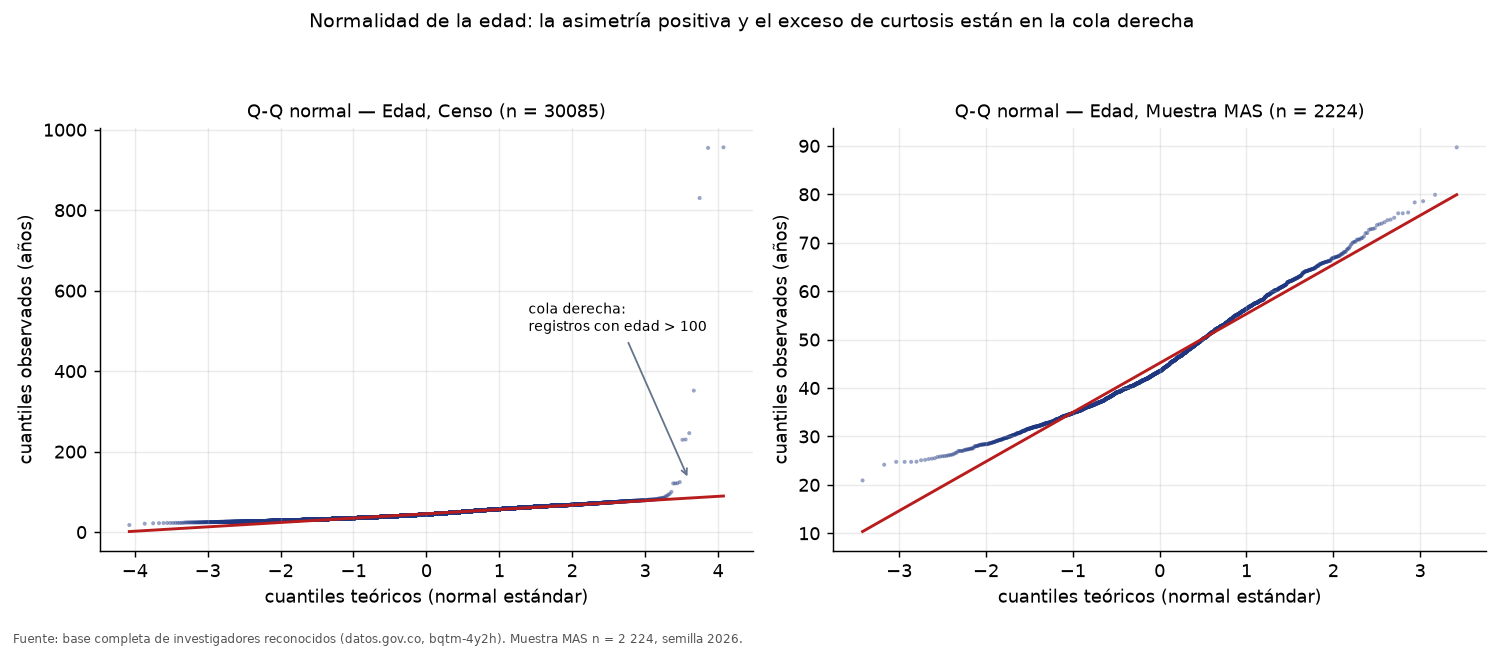
\includegraphics[width=0.78\textwidth]{figuras/07_qq_edad.png}
  \caption{Q-Q plot de la edad: censo y muestra. El censo se aparta en la cola
  por los registros con edad superior a 100 años.}
  \label{fig:mues-qq}
\end{figure}

\subsubsection{Heterocedasticidad del modelo GREG}

Modelo diagnosticado: la edad con auxiliares género, gran área y región
(2 224 observaciones, 17 parámetros).

\begin{table}[H]
  \centering
  \small
  \caption{Contrastes de heterocedasticidad del modelo de edad.}
  \label{tab:mues-heteroced}
  \begin{tabular}{@{}lrrrp{5.4cm}@{}}
    \toprule
    \textbf{Prueba} & \textbf{Estadístico} & \textbf{gl} & \textbf{$p$}
      & \textbf{Lectura} \\
    \midrule
    Breusch-Pagan & LM = 25,10 & 16 & 6,80e-02
      & \textbf{sin evidencia} de heterocedasticidad al 5 \% \\
    White (recortada) & LM = 62,12 & 136 & 1,00e+00 & degenerada: ver nota \\
    Levene entre celdas & 1,057 & --- & 3,52e-01 & \textbf{sin evidencia} \\
    Bartlett entre celdas & 59,99 & --- & 8,43e-01 & \textbf{sin evidencia} \\
    \bottomrule
  \end{tabular}
\end{table}

\textbf{Sobre la prueba de White: aquí no aplica limpiamente, y conviene explicar
por qué.} Con regresores \textbf{solo dicotómicos}, el cuadrado de una variable
dummy es la propia dummy y el producto cruzado de dos dummies es otra dummy. Los
términos adicionales que White introduce son por tanto colineales con los
niveles, y la matriz de diseño queda singular. Se ejecutó una versión recortada
(únicamente los 120 productos cruzados distintos): da LM = 62,1 con 136 grados de
libertad, un resultado degenerado que no aporta información. Lo apropiado con un
diseño factorial de este tipo es comparar las \textbf{varianzas entre las celdas
del modelo}, que es lo que hacen Levene y Bartlett, y ninguna de las dos
encuentra diferencias.

Queda un matiz honesto: la razón entre la varianza mayor y la menor de las celdas
es de 30,4$\times$, que en abstracto parece grande. La razón de que los contrastes
no la detecten es que las celdas con varianza extrema son muy pequeñas (la menor
tiene 5 observaciones), y un contraste no puede declarar una diferencia estable
con esa base. Se reportan las dos cosas en lugar de elegir la que conviene.

\textbf{¿Se justifican errores robustos?} No. El error estándar clásico de la
media ajustada es 1,1447 y el robusto HC3 es 1,1206: la razón es \textbf{0,979},
es decir la corrección robusta no solo no agranda el error sino que lo reduce
ligeramente. Con esa evidencia, un modelo con errores robustos añadiría
complejidad sin cambiar ninguna conclusión.

\textbf{El caso de la retención es distinto y hay que decirlo.} En una variable
binaria la heterocedasticidad es \textbf{estructural} ---$\text{Var}(y) = p(1-p)$
depende de $p$---, así que Breusch-Pagan la detecta siempre (LM = 125,1,
$p$ = 1,92e-10). No es un defecto del ajuste: es la razón por la que el GREG de la
retención se implementó con un modelo \textbf{logístico} y no con una
probabilidad lineal. Como comprobación de que la lineal no bastaba, sus valores
ajustados se salen del intervalo $[0,1]$: van de -0,028 a 1,126.

\begin{figure}[H]
  \centering
  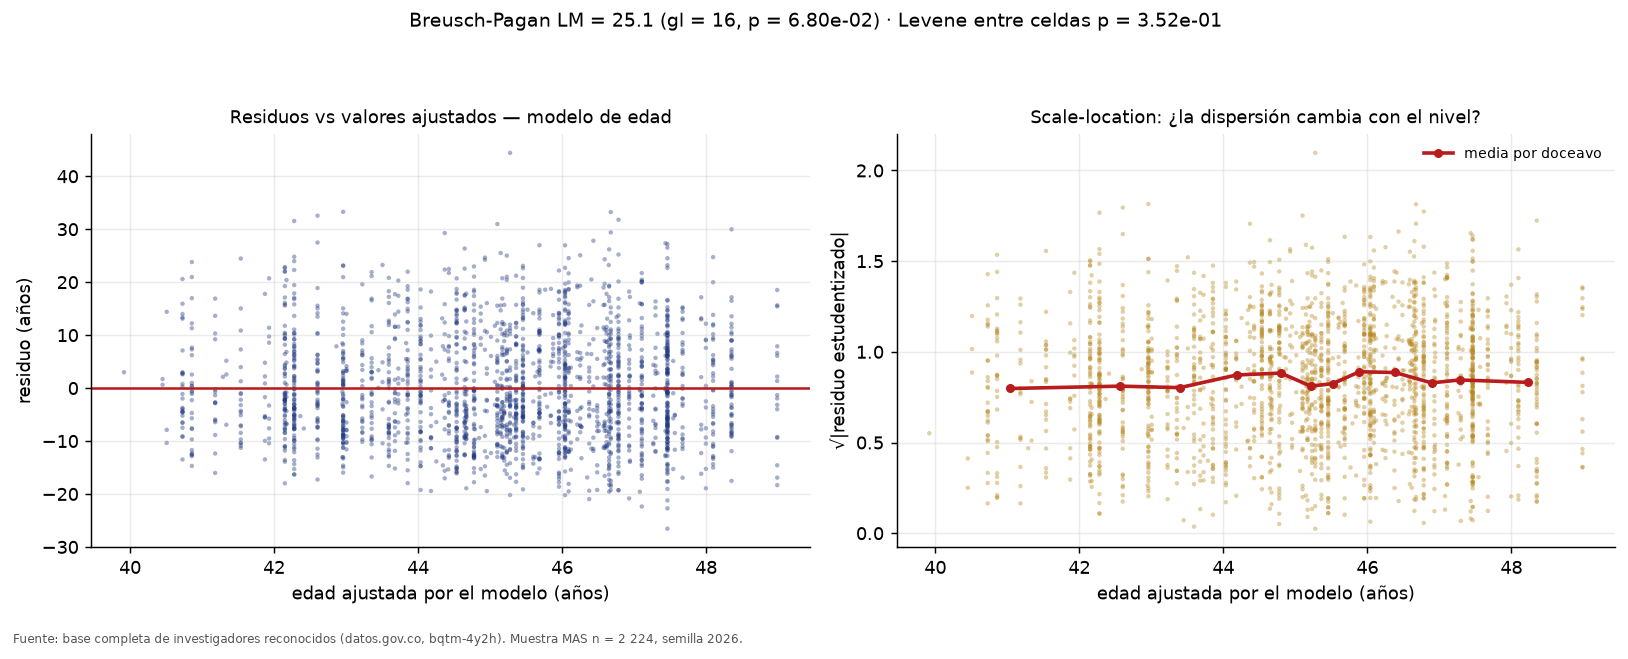
\includegraphics[width=0.78\textwidth]{figuras/08_residuos_vs_ajustados.png}
  \caption{Residuos frente a valores ajustados y scale-location del modelo de
  edad.}
  \label{fig:mues-residuos}
\end{figure}

\subsubsection{g-weights e influencia}

Los g-weights son los pesos implícitos que el GREG introduce sobre los pesos de
diseño: $w_i^{G} = w_i\,g_i$, con $g_i = 1 + \lambda' x_i$. Un g-weight grande
significa que unas pocas observaciones están cargando con toda la corrección del
modelo, y es la primera cosa que Hedlin et al. (2001) recomiendan mirar.

\begin{table}[H]
  \centering
  \footnotesize
  \caption{Distribución de los g-weights por modelo.}
  \label{tab:mues-gweights}
  \begin{tabular}{@{}lrrrrrrr@{}}
    \toprule
    \textbf{Modelo} & \textbf{Mínimo} & \textbf{q05} & \textbf{Mediana}
      & \textbf{q95} & \textbf{Máximo} & \textbf{$>$ 5} & \textbf{$>$ 10} \\
    \midrule
    Edad (género, área, región) & 0,584 & 0,827 & 1,020 & 1,103
      & \textbf{1,471} & 0 & 0 \\
    Retención 2019$\rightarrow$2021 (lineal) & 0,374 & 0,753 & 1,006 & 1,228
      & \textbf{2,696} & 0 & 0 \\
    \bottomrule
  \end{tabular}
\end{table}

\textbf{No hay ningún g-weight extremo}: el máximo es 1,471 en el modelo de edad y
2,696 en el de retención, muy por debajo de los umbrales de alarma de 5 y 10. La
media es exactamente 1, como debe ser. Adicionalmente se comprobó la propiedad de
calibración: $\sum w_i g_i = N$ se cumple de forma exacta (razón 1,000000).

\textbf{Un hallazgo que sí conviene declarar.} Los totales auxiliares se
reproducen exactamente \textbf{salvo una columna} de género, y por una razón de
diseño, no de cálculo: la categoría \emph{Otro / No especificado} tiene cero
observaciones en la muestra, así que ninguna observación la representa y su total
poblacional no es calibrable. La matriz de calibración tiene número de condición
5,2e+17 y rango 16 sobre 17 columnas. Es un límite del método frente a categorías
no representadas, y la solución ---si interesara--- sería de diseño: garantizar
representación de esas categorías. La sección~\ref{sec:mues-genero} lo
cuantifica.

Las demás columnas se reproducen con precisión de máquina (desvío máximo 4,0e-11
en las calibrables), y la masa que queda sin calibrar son 8 personas de 30 085,
es decir el 0,0266 \% del universo de esa población.

\textbf{Observaciones influyentes.} Leverage medio 0,0072 y máximo 0,0941;
distancia de Cook máxima \textbf{0,0223}. Aquí hay que leer los umbrales con
cuidado: superan el umbral de Cook ($4/n$ = 0,0018) 84 observaciones y el de
leverage ($2k/n$ = 0,0153) 103, pero el criterio convencional de preocupación es
Cook $> 1$ y el máximo observado es 0,0223: \textbf{dos órdenes de magnitud por
debajo}. Con $n$ grande esos umbrales señalizan muchas observaciones sin que
ninguna sea materialmente influyente. Lo que decide es la magnitud, no el
recuento.

Para no quedarse en la teoría, se recalculó el estimador GREG
\textbf{eliminando} las observaciones de $g$ más alto y se midió el efecto:

\begin{table}[H]
  \centering
  \small
  \caption{Sensibilidad del estimador de la edad a las observaciones con mayor $g$.}
  \label{tab:mues-sensibilidad}
  \begin{tabular}{@{}lrrr@{}}
    \toprule
    \textbf{Se eliminan} & \textbf{Estimador de la edad} & \textbf{Cambio}
      & \textbf{$g$ máximo restante} \\
    \midrule
    las 0 de mayor $g$ & 45,1528 & 0,00000 & 1,471 \\
    las 5 de mayor $g$ & 45,1423 & -0,01054 & 2,428 \\
    las 10 de mayor $g$ & 45,1110 & -0,04178 & 8,205 \\
    las 25 de mayor $g$ & 45,1705 & 0,01766 & 1,314 \\
    ninguna (completo) & 45,1528 & 0,00000 & 1,471 \\
    \bottomrule
  \end{tabular}
\end{table}

El efecto máximo de quitar las 25 observaciones con mayor $g$ es de 0,04178 años,
es decir \textbf{menos de un mes de edad media}: ninguna observación individual
está moviendo el resultado.

\begin{figure}[H]
  \centering
  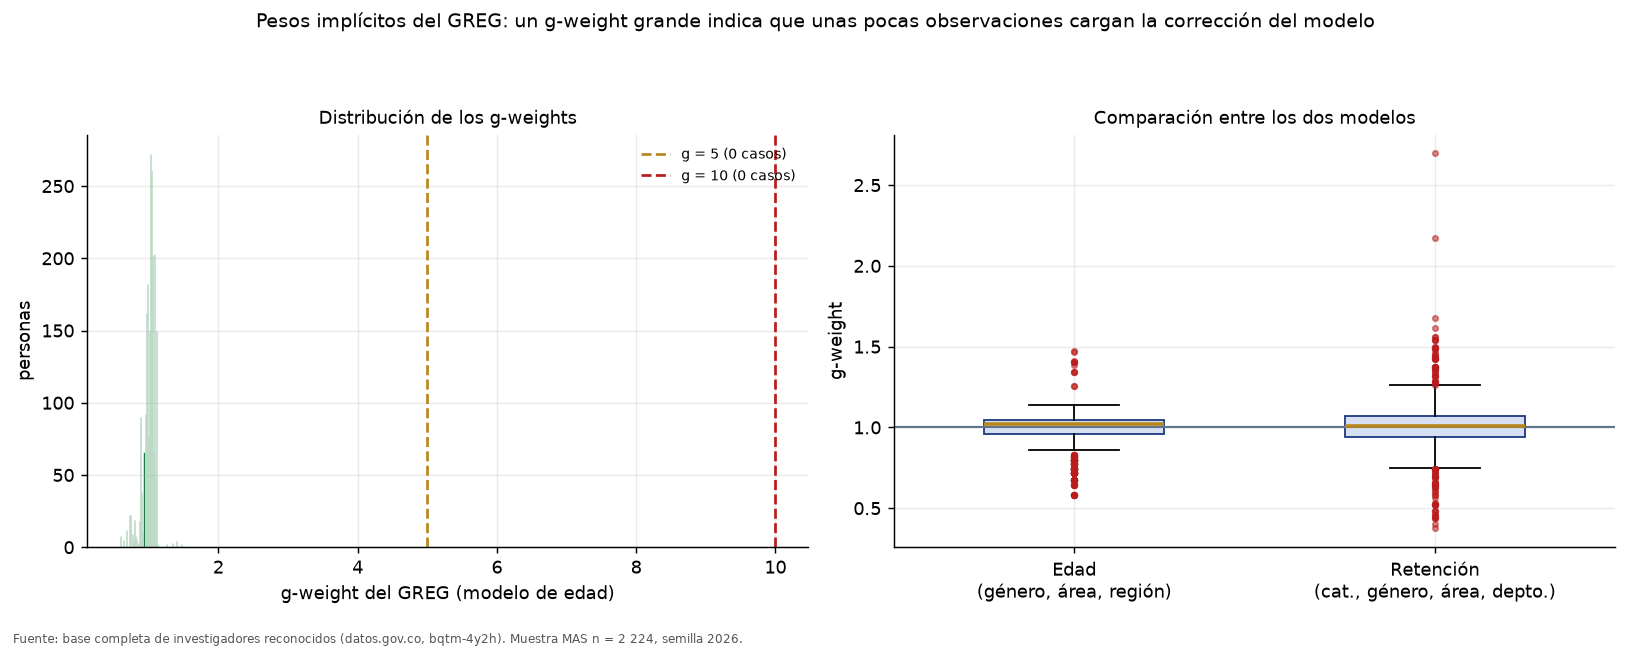
\includegraphics[width=0.78\textwidth]{figuras/09_gweights.png}
  \caption{Distribución de los g-weights del modelo de edad.}
  \label{fig:mues-gweights}
\end{figure}

\subsubsection{Colapso de las categorías de género no representadas}
\label{sec:mues-genero}

\textbf{El problema.} El registro reconoce cuatro categorías de género. Dos de
ellas tienen una presencia mínima en el universo y \textbf{ninguna} en la muestra:

\begin{table}[H]
  \centering
  \small
  \caption{Categorías de género con presencia mínima y su representación muestral.}
  \label{tab:mues-genero}
  \begin{tabular}{@{}lrrrr@{}}
    \toprule
    \textbf{Categoría} & \textbf{Personas en el censo} & \textbf{\% del censo}
      & \textbf{Registros} & \textbf{Observaciones en la muestra} \\
    \midrule
    Intersexual & 5 & 0,0166 \% & 5 & \textbf{0} \\
    No disponible & 4 & 0,0133 \% & 4 & \textbf{0} \\
    \emph{Otro / No especificado} (colapsada) & 9 & 0,0299 \% & --- & \textbf{0} \\
    \bottomrule
  \end{tabular}
\end{table}

Las \textbf{9 personas} son el 0,030 \% del censo. Un detalle que importa para lo
que sigue: las etiquetas \emph{Intersexual} y \emph{No disponible} aparecen
\textbf{únicamente en la convocatoria 2021} (5 y 4 registros, respectivamente).
Las mismas personas sí figuran en convocatorias anteriores, pero con otra etiqueta
de género.

\textbf{La consecuencia.} Una categoría auxiliar con cero observaciones en la
muestra no es calibrable: el GREG no puede reproducir su total poblacional porque
ninguna observación lo representa, y su coeficiente queda indeterminado. No es un
error de cálculo; es un límite del diseño. En la comprobación de calibración
aparecía como un desvío exactamente igual al recuento censal de la columna (8
personas sin calibrar, repartidas en dos columnas). Son 8 y no 9 porque el modelo
de edad excluye a la persona sin edad registrada, que es una de las 9 colapsadas.

\textbf{La decisión.} En \textbf{todos los análisis desagregados por género} las
dos categorías se colapsan en una sola, \emph{Otro / No especificado}. Se conserva
la columna original del registro para dos usos que sí necesitan el dato crudo: el
control de calidad de género contradictorio (que cuenta categorías distintas por
persona y por eso debe ver el registro tal como está) y el visor de trayectorias,
que reproduce el censo sin transformarlo.

\textbf{Qué cambia y qué no.} Se midieron tres variantes del vector auxiliar del
modelo de edad. Los estimadores son idénticos en las tres:

\begin{table}[H]
  \centering
  \scriptsize
  \caption{Variantes del vector auxiliar de género y su efecto sobre la calibración.}
  \label{tab:mues-variantes-genero}
  \begin{tabular}{@{}p{4.6cm}rrrrrr@{}}
    \toprule
    \textbf{Variante} & \textbf{Cols.} & \textbf{Rango(M)} & \textbf{cond(M)}
      & \textbf{No calibrables} & \textbf{Sin calibrar} & \textbf{GREG edad} \\
    \midrule
    Sin colapsar (4 categorías crudas) & 18 & 16 de 18 & 2,3e+17 & 2 & 8 & 45,1528 \\
    \textbf{Colapsada (decisión adoptada)} & 17 & 16 de 17 & 5,2e+17 & 1 & 8 & 45,1528 \\
    Colapsada y columna excluida & 16 & 16 de 16 & 3,9e+02 & 0 & 0 & 45,1528 \\
    \bottomrule
  \end{tabular}
\end{table}

El colapso \textbf{no devuelve la calibrabilidad} a la categoría: la causa es la
ausencia en la muestra, no la granularidad excesiva. Reduce de dos a una las
columnas no calibrables y agrupa el hueco en un rótulo, pero la masa sin calibrar
sigue siendo de 8 personas y el rango de M no mejora. Tampoco empeora el ajuste:
el desvío de esa columna es exactamente su recuento censal y las demás se
reproducen con precisión de máquina.

Dos consecuencias verificadas que conviene dejar dichas, porque podrían esperarse
mal:

\begin{enumerate}
  \item \textbf{El estimador y su varianza no cambian en absoluto} (diferencia 0
        años entre colapsar y no colapsar). Era previsible: en la muestra ambas
        columnas eran constantes cero, así que su coeficiente ya era nulo y el
        colapso solo fusiona dos columnas nulas en una. El colapso es una decisión
        de \textbf{coherencia y trazabilidad}, no una corrección numérica, y así
        se reporta.
  \item \textbf{Las tablas de retención y transición por género no cambian.} La
        convocatoria base de cada par es siempre anterior a 2021, y las etiquetas
        solo existen en 2021: ninguna persona aparece con ellas como base de un
        par. Se comprobó sobre los resultados del panel y no hay ni una sola celda
        de las tablas desagregadas por género que las contenga. Lo que sí cambia
        es la prueba de representatividad, y solo en los grados de libertad: el
        estadístico es invariante ($\chi^2$ = 3,1283 en ambos casos, porque una
        celda con observado cero aporta a $\chi^2$ exactamente su esperado),
        mientras los gl bajan de 3 a 2 y el $p$-valor sube de 0,3723 a 0,2093. Con
        el colapso la distribución de género de la muestra sigue siendo compatible
        con la del censo, y el supuesto de frecuencia esperada mínima sigue sin
        cumplirse en ninguno de los dos casos (esperado mínimo 0,6653 $<$ 5).
  \item \textbf{Los diagnósticos que se normalizan por el número de parámetros sí
        se mueven, y en la proporción esperada.} La distancia de Cook máxima pasa
        de 0,0211 a 0,0223: el factor es el cociente de parámetros
        (18/17 = 1,0588), porque la fórmula de Cook divide por $k$, más el ajuste
        de $n-k$ en la varianza residual. El ajuste no cambia ---los residuos son
        los mismos--- pero conviene decirlo para que la diferencia no parezca un
        efecto del colapso sobre el modelo.
\end{enumerate}

\begin{figure}[H]
  \centering
  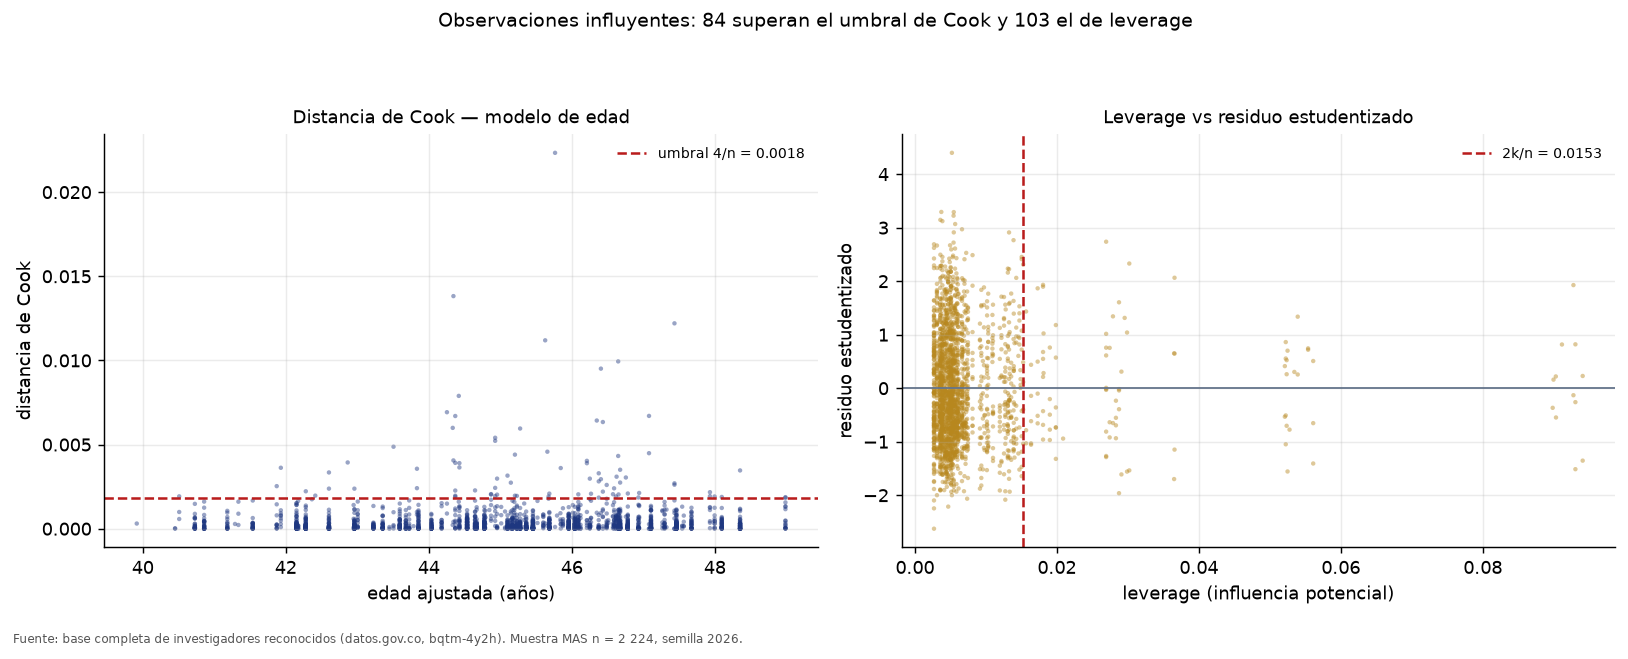
\includegraphics[width=0.78\textwidth]{figuras/10_influencia.png}
  \caption{Distancia de Cook y leverage del modelo de edad. El máximo de Cook
  (0,0223) está dos órdenes de magnitud por debajo del umbral de preocupación.}
  \label{fig:mues-influencia}
\end{figure}

\textbf{La limitación que permanece, y su salida.} La categoría colapsada sigue
sin ser calibrable, así que los totales auxiliares no se reproducen al 100 \%. Si
se quisiera cerrar el hueco por completo hay dos caminos, y ninguno es un truco de
cálculo: (i) \textbf{de diseño}, garantizar representación de esas categorías en
la muestra; o (ii) \textbf{de alcance}, excluir del vector auxiliar la columna no
representada y declarar que el género de esas 8 personas queda fuera de la
calibración. La tercera fila de la tabla~\ref{tab:mues-variantes-genero} mide la
variante (ii): deja \textbf{cero} columnas sin calibrar y un número de condición
de 3,9e+02 ---frente a 5,2e+17--- con el \textbf{mismo estimador}. No se adoptó
porque la decisión acordada es colapsar y declarar, y porque dejar la columna
dentro hace visible la limitación en la propia comprobación de calibración; pero
está medida y disponible si se prefiere la calibración exacta.

\subsubsection{Conclusión: ¿es razonable el modelo GREG?}

\textbf{Sí, con dos matices documentados.} La evidencia:

\begin{enumerate}
  \item \textbf{Sin g-weights extremos.} Máximo 1,471 (edad) y 2,696 (retención);
        ninguno supera 5. La calibración se verifica exactamente
        ($\sum w_i g_i = N$).
  \item \textbf{Sin observaciones influyentes materiales.} Distancia de Cook
        máxima 0,0223, muy por debajo del nivel de preocupación; quitar las
        observaciones de mayor $g$ mueve la estimación menos de 0,05 años.
  \item \textbf{Sin heterocedasticidad que exija corrección.} Breusch-Pagan
        $p$ = 6,80e-02, Levene $p$ = 3,52e-01, Bartlett $p$ = 8,43e-01; y la razón
        HC3/clásico de 0,979 confirma que los errores robustos no aportan.
  \item \textbf{La normalidad no es un supuesto crítico.} No se cumple en el
        censo por 11 edades erróneas, pero la consistencia del GREG es por diseño
        y no depende de ella.
\end{enumerate}

\textbf{Los dos matices.} Primero, la categoría de género \emph{Otro / No
especificado} no es calibrable porque no tiene representación en la muestra: el
límite está en el diseño muestral, no en el estimador, y se declara en lugar de
omitirse (ver la sección~\ref{sec:mues-genero}, donde además se mide la variante
que sí calibra exactamente). Segundo, la prueba de White no es aplicable a un
diseño de solo dicotómicas y se sustituye por contrastes de homocedasticidad entre
celdas, que es lo apropiado para un modelo factorial. Con esas salvedades, los
diagnósticos respaldan el uso del GREG que se reporta en las
secciones~\ref{sec:mues-greg} y~\ref{sec:mues-comparacion}.

% =====================================================================
\subsection{Conclusión: qué se reporta y por qué}
\label{sec:mues-conclusion}

\begin{enumerate}
  \item \textbf{Las cifras oficiales del análisis longitudinal son las del
        censo.} La base completa está disponible, así que no hay razón para
        reportar una estimación cuando se puede reportar el parámetro. Toda la
        maquinaria de muestreo de esta sección tiene un valor
        \textbf{metodológico y de verificación}, no de sustitución.
  \item \textbf{Si hubiera que estimar a partir de la muestra, el MAS simple ya
        sería suficiente y es el que menos supuestos exige.} Es insesgado por
        diseño y en esta aplicación resultó el más cercano al censo en 4 de los 6
        pares, precisamente porque la muestra quedó equilibrada.
  \item \textbf{La post-estratificación por categoría no corrige sesgo: compra
        precisión.} Reduce la varianza entre 0,6 \% y 16,6 \% según el par, sin
        mejorar de forma sistemática el error frente al censo. Se justifica cuando
        el objetivo es estrechar intervalos, no cuando se sospecha un desbalance.
  \item \textbf{El GREG es el estimador recomendado si hay que estimar}, porque
        domina en varianza (hasta 20,1 \% de reducción) y porque su validez no
        depende de que el modelo esté bien especificado: es la propiedad
        \emph{model-assisted} de Kalton (2002) y del FCSM (2003). Además resuelve
        el problema del estrato pequeño, que es el punto débil de la
        post-estratificación en este corpus.
  \item \textbf{El estrato pequeño se declara, no se esconde.} Con Emérito en 1,
        7 y 3 observaciones según el par, la post-estratificación de 4 estratos
        incumple la condición de tamaño mínimo de Cochran (1977). La versión
        colapsada (Sénior + Emérito) la cumple y se reporta junto a la otra, y el
        GREG ofrece una tercera vía que no depende de que cada celda sea grande.
\end{enumerate}

\textbf{Recomendación operativa.} Reportar el censo; documentar el MAS como el
diseño de referencia y su validación (Anexo A de
\texttt{analisis\_longitudinal.md}); y usar GREG ---no la post-estratificación de
4 estratos--- si en algún momento hubiera que producir una estimación muestral con
intervalos más estrechos.

% =====================================================================
\subsection*{Referencias de esta sección}
\addcontentsline{toc}{subsection}{Referencias de esta sección}

{\sloppy
\begin{itemize}
  \item Cochran, W. G. (1977). \emph{Sampling Techniques} (3rd ed.). John Wiley
        \& Sons. --- Formulación y ajuste del tamaño de muestra;
        post-estratificación (\S5A); recomendación de 4 a 6 estratos con
        $\sim$20 observaciones por estrato (pp.~132--134).
  \item Lohr, S. L. (2010). \emph{Sampling: Design and Analysis} (2nd ed.).
        Brooks/Cole. --- Muestreo aleatorio simple, estimación de proporciones y
        post-estratificación (\S7.6).
  \item Särndal, C.-E., Swensson, B., \& Wretman, J. (1992). \emph{Model Assisted
        Survey Sampling}. Springer-Verlag. --- Estimador GREG y su forma de
        diferencia (\S6.4--6.5); la post-estratificación como caso particular con
        modelo saturado.
  \item Kalton, G. (2002). Models in the practice of survey sampling.
        \emph{International Statistical Review}, 70(2), 175--192. --- Uso de
        modelos en modo asistido, de forma que la validez de las estimaciones no
        dependa de los supuestos del modelo.
  \item FCSM (2003). \emph{Glossary of Terms}. Federal Committee on Statistical
        Methodology. --- Definición y motivación del estimador GREG como
        \emph{model-assisted}.
  \item StatsRef.com (s.~f.). \emph{Exploratory data analysis}. En
        \emph{Statistics Reference Online}. --- «EDA \dots{} is typically the
        first stage of any such analysis»; síntesis de la posición de Cochran
        (1977) sobre el trabajo exploratorio previo.
  \item OhioLINK ETD Center. \emph{Post-stratification variance}. --- La
        distribución asintótica del estimador post-estratificado coincide con la
        del estimador de un muestreo estratificado con asignación proporcional
        (Cochran, 1977; Lohr, 1999).
  \item Canadian Journal of Forest Research (2019). \emph{Efficiency of
        post-stratification for a large-scale forest inventory}. --- Recomendación
        de Cochran (1977, pp.~132--134) sobre el número de estratos y el tamaño
        mínimo por estrato.
  \item Hedlin, D., y Falvey, H. \emph{Does the model matter for GREG estimation?
        A business survey example}. --- Análisis de g-weights, residuos y
        diagnósticos de regresión para verificar que una estimación GREG es
        razonable. Nota de transparencia: la ficha se verificó por búsqueda en
        línea (Semantic Scholar y DiVA, Universidad de Estocolmo), pero el año
        (2001) procede del enunciado de la tarea: el metadato accesible no
        permitió confirmarlo en el entorno de trabajo.
  \item Valliant, R. et al. \emph{svydiags: Regression Model Diagnostics for
        Survey Data} [paquete de R]. CRAN. --- Diagnósticos de regresión
        (residuos, leverage, influencia) adaptados a datos de encuesta.
  \item Field, A. (2009). \emph{Discovering Statistics Using SPSS} (3rd ed.).
        SAGE. --- Recomendación de usar asimetría y curtosis como criterio
        principal de normalidad cuando $n > 200$.
\end{itemize}
}

% =====================================================================
\subsection*{Artefactos y reproducibilidad}
\addcontentsline{toc}{subsection}{Artefactos y reproducibilidad}

\begin{table}[H]
  \centering
  \small
  \caption{Artefactos que producen las cifras de esta sección.}
  \label{tab:mues-artefactos}
  \begin{tabular}{@{}p{7.2cm}p{7.6cm}@{}}
    \toprule
    \textbf{Artefacto} & \textbf{Contenido} \\
    \midrule
    \texttt{src/eda\_longitudinal.py} & EDA completo (parte 1) \\
    \texttt{data/memoria/eda\_resultados.json} & Cifras del EDA \\
    \texttt{data/memoria/eda/} & 6 gráficas del EDA \\
    \texttt{src/estimadores\_longitudinal.py} & Post-estratificación y GREG
      (partes 2--3) \\
    \texttt{data/memoria/estimadores\_resultados.json} & Cifras de los estimadores \\
    \texttt{src/genero\_comun.py} & Colapso de las categorías de género \\
    \texttt{src/diagnosticos\_greg.py} & Diagnósticos de supuestos y g-weights \\
    \texttt{data/memoria/diagnosticos\_greg.json} & Cifras de los diagnósticos \\
    \texttt{data/memoria/eda/07\_qq\_edad.png} & Q-Q plot de la edad \\
    \texttt{data/memoria/eda/08\_residuos\_vs\_ajustados.png} & Residuos frente a
      ajustados \\
    \texttt{data/memoria/eda/09\_gweights.png} & Distribución de los g-weights \\
    \texttt{data/memoria/eda/10\_influencia.png} & Distancia de Cook y leverage \\
    \texttt{src/generar\_metodologia\_muestreo.py} & Genera el informe de origen \\
    \bottomrule
  \end{tabular}
\end{table}

\begin{verbatim}
python src/eda_longitudinal.py
python src/estimadores_longitudinal.py
python src/diagnosticos_greg.py
python src/generar_metodologia_muestreo.py
\end{verbatim}

El muestreo \textbf{no se rehizo}: se reutilizan los identificadores de
\texttt{data/memoria/muestra\_ids.csv} (semilla 2026).
